%% TRANSVRP manuscript — INFORMS Transportation Science submission template
%% Build: python make_tables.py && pdflatex transvrp && bibtex transvrp && pdflatex transvrp && pdflatex transvrp
%% Every result number in the text comes from numbers.tex and every table from
%% tables/*.tex, both written by make_tables.py from the committed result files.
%% Protocol facts (counts of routes, gate outcomes, tuning grids) come from
%% RESEARCH_LOG.md and the pre-registrations EXPERIMENT_A.md / EXPERIMENT_B.md.

\documentclass[trsc,dblanonrev]{informs4}
\usepackage{eqndefns-left}
\RequirePackage{tgtermes}
\RequirePackage{mathptmx}
\RequirePackage{bm}
\usepackage{booktabs}
\usepackage{graphicx}
\usepackage{amsmath}

\OneAndAHalfSpacedXII

\usepackage{natbib}
 \bibpunct[, ]{(}{)}{,}{a}{}{,}%
 \def\bibfont{\footnotesize}%
 \def\bibsep{1pt plus 1pt minus 1pt}%
 \def\bibhang{24pt}%
 \def\newblock{\ }%
 \def\BIBand{and}%

\setlength\floatsep{10pt plus 4pt minus 4pt}
\setlength\textfloatsep{12pt plus 4pt minus 4pt}
\setlength\intextsep{10pt plus 4pt minus 4pt}

\EquationsNumberedThrough
\TheoremsNumberedThrough

\MANUSCRIPTNO{TRSC-0000-2026.00}

\newcommand{\Full}{\textsc{Full}}
\newcommand{\Scalar}{\textsc{Scalar}}
\newcommand{\Mlp}{\textsc{Mlp}}
\newcommand{\Boost}{\textsc{Boost}}
\newcommand{\Baton}{\textsc{Baton}}
\newcommand{\Thr}{\textsc{Thr}}
\newcommand{\Alpz}{\textsc{Alp-Z}}
\newcommand{\Rlsm}{\textsc{Rlsm}}
\newcommand{\Dqn}{\textsc{Dqn}}
\newcommand{\Ppo}{\textsc{Ppo}}
\newcommand{\Dos}{\textsc{Dos}}
% generated by make_tables.py; do not edit
\newcommand{\APrim}{+0.82\%}
\newcommand{\APrimCI}{[+0.65, +0.99]}
\newcommand{\APrimCIn}{[+0.68, +0.96]}
\newcommand{\APrimBetter}{19/20}
\newcommand{\ASone}{-1.34\%}
\newcommand{\ASoneCI}{[-2.34, -0.33]}
\newcommand{\ASoneCIn}{[-2.17, -0.51]}
\newcommand{\ASoneBetter}{5/20}
\newcommand{\AStwo}{+0.11\%}
\newcommand{\AStwoCI}{[-0.40, +0.63]}
\newcommand{\AStwoCIn}{[-0.31, +0.54]}
\newcommand{\AStwoBetter}{15/20}
\newcommand{\ASthree}{+0.42\%}
\newcommand{\ASthreeCI}{[+0.25, +0.59]}
\newcommand{\ASthreeCIn}{[+0.28, +0.56]}
\newcommand{\ASthreeBetter}{17/20}
\newcommand{\ASfour}{+0.61\%}
\newcommand{\ASfourCI}{[+0.45, +0.77]}
\newcommand{\ASfourCIn}{[+0.48, +0.75]}
\newcommand{\ASfourBetter}{19/20}
\newcommand{\ASfive}{+0.83\%}
\newcommand{\ASfiveCI}{[+0.66, +0.99]}
\newcommand{\ASfiveCIn}{[+0.69, +0.96]}
\newcommand{\ASfiveBetter}{20/20}
\newcommand{\ASsix}{+0.45\%}
\newcommand{\ASsixCI}{[+0.32, +0.59]}
\newcommand{\ASsixCIn}{[+0.34, +0.56]}
\newcommand{\ASsixBetter}{19/20}
\newcommand{\ASseven}{+0.07\%}
\newcommand{\ASsevenCI}{[-0.02, +0.16]}
\newcommand{\ASsevenCIn}{[-0.00, +0.14]}
\newcommand{\ASsevenBetter}{10/20}
\newcommand{\ASeight}{-0.04\%}
\newcommand{\ASeightCI}{[-0.19, +0.12]}
\newcommand{\ASeightCIn}{[-0.16, +0.09]}
\newcommand{\ASeightBetter}{9/20}
\newcommand{\ASnine}{+0.31\%}
\newcommand{\ASnineCI}{[+0.21, +0.40]}
\newcommand{\ASnineCIn}{[+0.23, +0.38]}
\newcommand{\ASnineBetter}{20/20}
\newcommand{\ASten}{+0.76\%}
\newcommand{\AStenCI}{[+0.58, +0.93]}
\newcommand{\AStenCIn}{[+0.61, +0.90]}
\newcommand{\AStenBetter}{19/20}
\newcommand{\ASeleven}{+0.90\%}
\newcommand{\ASelevenCI}{[+0.71, +1.08]}
\newcommand{\ASelevenCIn}{[+0.75, +1.05]}
\newcommand{\ASelevenBetter}{20/20}
\newcommand{\ABoost}{+0.25\%}
\newcommand{\ABoostCI}{[+0.17, +0.34]}
\newcommand{\ABoostCIn}{[+0.19, +0.32]}
\newcommand{\ABoostBetter}{20/20}
\newcommand{\BAlpz}{+11.33\%}
\newcommand{\BAlpzCI}{[+8.76, +13.91]}
\newcommand{\BAlpzCIn}{[+9.21, +13.46]}
\newcommand{\BAlpzBetter}{20/20}
\newcommand{\BAlpzVsBaton}{-13.62\%}
\newcommand{\BRlsm}{+0.16\%}
\newcommand{\BRlsmCI}{[+0.09, +0.24]}
\newcommand{\BRlsmCIn}{[+0.10, +0.22]}
\newcommand{\BRlsmBetter}{17/20}
\newcommand{\BRlsmVsBaton}{+0.69\%}
\newcommand{\BDqn}{+0.16\%}
\newcommand{\BDqnCI}{[+0.11, +0.21]}
\newcommand{\BDqnCIn}{[+0.11, +0.20]}
\newcommand{\BDqnBetter}{19/20}
\newcommand{\BDqnVsBaton}{+0.70\%}
\newcommand{\BPpo}{+1.68\%}
\newcommand{\BPpoCI}{[+0.46, +2.90]}
\newcommand{\BPpoCIn}{[+0.67, +2.69]}
\newcommand{\BPpoBetter}{20/20}
\newcommand{\BPpoVsBaton}{-1.12\%}
\newcommand{\BThr}{+11.01\%}
\newcommand{\BThrCI}{[+8.48, +13.54]}
\newcommand{\BThrVsBaton}{-13.16\%}
\newcommand{\AvsFULL}{+0.82\%}
\newcommand{\AvsSCALAR}{0.00\%}
\newcommand{\AvsMLP}{+0.52\%}
\newcommand{\AvsBOOST}{+0.57\%}
\newcommand{\AvsBATONrich}{+0.29\%}
\newcommand{\BIndBaton}{+0.09\%}
\newcommand{\BIndBatonCI}{[-0.39, +0.56]}
\newcommand{\BIndThr}{-0.01\%}
\newcommand{\BIndThrCI}{[-0.31, +0.28]}
\newcommand{\BIndAlpz}{-0.03\%}
\newcommand{\BIndAlpzCI}{[-0.35, +0.28]}
\newcommand{\BIndNone}{+12.25\%}
\newcommand{\BIndNoneCI}{[+7.82, +16.67]}
\newcommand{\Crossover}{500}
\newcommand{\Margin}{0.7\%}
\newcommand{\BReEval}{+0.85\%}
\newcommand{\BReEvalCI}{[+0.68, +1.02]}
\newcommand{\ThrAlpzGap}{0.39\%}
\newcommand{\AvsSCALARCIn}{[-0.04, +0.04]}
\newcommand{\ShareMlp}{37\%}
\newcommand{\ShareBoost}{31\%}
\newcommand{\ShareRlsm}{19\%}
\newcommand{\ShareDqn}{18\%}
\newcommand{\RepSdFull}{0.11\%}
\newcommand{\RepSdBaton}{0.13\%}
\newcommand{\RepSdRlsm}{0.11\%}
\newcommand{\RepSdDqn}{0.16\%}
\newcommand{\RepSdPpo}{0.37\%}
\newcommand{\PpoHours}{5.9}
\newcommand{\FullMinutesB}{32}


\begin{document}

\RUNAUTHOR{Anonymous}

\RUNTITLE{What the Driver Knows}

\TITLE{What the Driver Knows: State Information, Not the Learner, Drives
Learned Recourse in Vehicle Routing with Stochastic Pickups and Deliveries}

\ARTICLEAUTHORS{%
\AUTHOR{Author names blinded for peer review}
\AFF{Affiliations blinded for peer review}
}

\ABSTRACT{%
A vehicle on a planned route with simultaneous pickups and deliveries must
decide after each stop whether to continue or to hand the remaining stops to
a standby vehicle before its load exceeds capacity. This is an optimal-stopping
problem, and many learning methods could solve it. We ask which ingredient
matters: the information in the state or the learner. In two pre-specified
experiments on 62 routes of 20 Dethloff instances, every method is trained on
the same $10^5$ simulated paths per route and tested on a held-out stream of
20{,}000 days, with the instance as the unit of analysis. A regression policy
that observes pickups and deliveries separately lowers recourse cost by
0.82\% (95\% CI 0.65 to 0.99) relative to Longstaff--Schwartz regression on
the net load, and the gain vanishes when the same network sees only the load.
On the rich state, a perceptron, boosted trees, randomized networks and double
deep Q-learning come within 0.16 to 0.31 points of the transformer, inside a
pre-specified equivalence margin of 0.7\%; the learner changes cost by less than
40\% of what the state changes. Two published methods that compute
the continuation value from per-stop marginals under an independence
assumption are about 13\% dearer than the regression policy on the load, and
the gap disappears when stops are made independent. Our adaptation of proximal
policy optimization falls short at its source's training budget. The rich state
stops losing to the scalar policy at about 500 training paths per route and
gains steadily beyond. The practical lesson is to record what the driver
already observes and to fit the simplest regressor that uses it.}

\KEYWORDS{stochastic vehicle routing; pickup and delivery; recourse; optimal
stopping; approximate dynamic programming; reinforcement learning; regression
Monte Carlo}

\maketitle

%% ==========================================================================
\section{Introduction}\label{sec:intro}

A routing plan fixes the sequence of customers; the day then reveals how much
each customer hands over and takes back. With simultaneous pickups and
deliveries the load is not monotone: it falls at a delivery and rises at a
pickup, and an overflow can occur at any stop. An operator with a standby
fleet can avoid an overflow by handing the rest of the route to a standby
vehicle, at a known price, before the breach happens. Waiting too long costs an
emergency hire and late customers; handing off too early wastes the standby
vehicle. The decision is an optimal-stopping problem along the route
\citep{dang2026baton}.

Many methods could make this decision: threshold dynamic programs
\citep{yang2000stochastic, venkateshan2026note}, approximate linear programs
for outsourcing recourse \citep{zhu2026partial}, regression Monte Carlo with
randomized neural networks \citep{herrera2024optimal}, deep Q-learning
\citep{dastpak2023offline}, policy-gradient methods with graph encoders
\citep{kadyrov2025drl}, and transformers trained for real-time decisions
\citep{liu2026ortransformer}. These methods differ in two things at once: what
the policy observes and how it learns. A practitioner choosing among them needs
to know which of the two matters, and the published comparisons cannot say,
because each method is evaluated on its own data, state and problem.

We separate the two by design. Every method is trained on the same simulated
paths, deployed through the same simulator and evaluated on the same held-out
days; methods differ in the state they observe, in the learner, or in both, and
the design names which. The reference policy is \Baton{}
\citep{dang2026baton}, which estimates the cost of continuing by
Longstaff--Schwartz regression \citep{longstaff2001valuing} on the net load
with an isotonic regressor. We pair it with \Full{}, which runs the same
backward induction but regresses on what the driver has actually seen:
pickups and deliveries separately, their deviations from historical means,
and a summary of the stops still ahead. Two pre-specified experiments then ask
three questions. Does the rich state pay (experiment A)? Is any gain due to the
information or to the network (A, by ablation)? Does the conclusion survive
against published methods of 2023--2026 (experiment B)?

In short: the rich state pays, by \APrim{} of recourse cost at $10^5$ paths
per route; the gain is information, because the same network without the
history features gains nothing and four other learners on the rich state are
equivalent to it; and the large losses of two published methods come from
their independence assumption, not from their state.

Our contributions are as follows. (i) A controlled comparison of nine methods
for in-route recourse on identical data, with decision rules fixed in advance,
a held-out test stream per experiment, and Holm-adjusted inference at the
instance level. (ii) An attribution of the improvement over the scalar policy
to state information, through ablations that hold the learner fixed and
learners that hold the state fixed. (iii) A separation of two sources of loss
that the literature conflates: a load-only state costs \Baton{} under 1\%,
while computing the continuation value under an independence assumption costs
about 13\%; an independence-permuted world removes the latter. (iv) A
data-size curve showing where the rich state starts to pay. (v) A protocol
(development gates, model manifests, a family line hashed before the test
stream is read) for comparisons of learned recourse; code and results are
released with the paper.

The scope is narrow by design: recourse cost on fixed routes, one demand
generator family (gamma marginals with Gaussian copulas) on the Dethloff
instances, and published methods adapted to a two-action problem.
Section~\ref{sec:limits} states what this does and does not license.

%% ==========================================================================
\section{Related Work}\label{sec:related}

\paragraph{Recourse in stochastic vehicle routing.} Since
\citet{bertsimas1992vehicle}, the a priori route with recourse has been the
standard model of the vehicle routing problem with stochastic demands (VRPSD);
see \citet{gendreau1996stochastic} and \citet{oyola2018stochastic} for surveys.
\citet{yang2000stochastic} introduced preventive restocking and showed that
along a fixed route the optimal policy has a threshold in the remaining load;
\citet{venkateshan2026note} re-establish threshold optimality for a fixed-route
model with delivery choice. \citet{louveaux2009one} study the one-commodity
pickup-and-delivery problem with stochastic demands, and
\citet{louveaux2018exact} give an exact approach with preventive returns.
Reoptimization, approximate dynamic programming and rollout
\citep{secomandi2009reoptimization, novoa2009approximate,
goodson2016restocking} let the route itself change. Recent planning work
revisits modelling choices \citep{hoogendoorn2025evaluation}, fairness under
partial deliveries \citep{kinable2026fair}, drone restocking
\citep{wang2025truckdrone}, optional pickups \citep{gobbi2026optional} and
learning-assisted matheuristics \citep{reynal2026hybrid}. Most of this
literature models demands as independent across customers or summarises the
state by the load. Our instances follow the benchmark protocol of
\citet{dang2026baton}, in which demands are correlated through common factors;
there the load is not a sufficient statistic, and a policy that observes more
can gain.

\paragraph{Value-function approximation for recourse.}
\citet{zhu2026partial} replace failure recourse by partial outsourcing and
derive a price-directed policy from an approximate linear program (ALP) whose
basis is indexed by location and load. It is the closest published analogue of
the handoff; on a fixed route their ALP becomes the exact linear program of the
independent-demand dynamic program (Section~\ref{sec:arms}).
\citet{dastpak2023offline} learn an offline value function for stochastic
demands with double Q-learning on a fixed-size observation, and a 2026
preprint extends the approach to outsourcing with a graph attention encoder
\citep{dastpak2026deep}. \citet{kadyrov2025drl} train a graph-encoder policy
with proximal policy optimization for dynamic routing under demand and traffic
uncertainty, and \citet{akkerman2025comparison} compare neural and linear
reinforcement-learning policies in dynamic routing. Surveys of learning for
combinatorial and dynamic routing are \citet{bengio2021machine} and
\citet{soeffker2022stochastic}; \citet{powell2011approximate} covers
approximate dynamic programming.

\paragraph{Optimal stopping by regression.} The least-squares Monte Carlo
method of \citet{longstaff2001valuing} and the analysis of
\citet{tsitsiklis2001regression} underlie \Baton{} and \Full{}.
\citet{herrera2024optimal} replace the regression basis by a randomized neural
network whose hidden layer is drawn at random and whose output layer is solved
by least squares; \citet{becker2019deep} learn the stopping decision directly
with a neural network. A recent preprint reports that simple regressors
(nearest neighbours, trees, linear models) match neural networks inside
regression methods for optimal switching \citep{andersson2026effectiveness};
experiment A points the same way for routing recourse.

\paragraph{Neural routing.} Attention-based constructive models
\citep{kool2019attention, nazari2018reinforcement, kwon2020pomo}, built on the
transformer \citep{vaswani2017attention}, learn to construct routes.
\citet{liu2026ortransformer} argue that permutation-equivariant transformers
trained with pathwise gradients scale real-time decisions in stochastic joint
replenishment. \Full{} uses such an encoder over the remaining stops, which
lets us test whether the architecture is what buys the improvement.

%% ==========================================================================
\section{Problem}\label{sec:problem}

\paragraph{Route and load.} A planned route visits customers $1,\dots,m$ in a
fixed order. At stop $j$ the vehicle delivers $d_j \ge 0$ and collects
$p_j \ge 0$, both observed on service. Let $g_j = p_j - d_j$ and let
$W_k = \sum_{j \le k} g_j$ ($W_0 = 0$) be the cumulative net load change after
stop $k$, which we call the net load. The vehicle departs with the planned
deliveries and overflows when $W_k$ exceeds the slack $B$ (capacity minus
departure load). The breach time is $\tau = \min\{k : W_k > B\}$, with
$\tau = m+1$ if no breach occurs.

\paragraph{Decision and cost.} After serving stop $k < \tau$,
$k = 1,\dots,m-1$, the driver either continues or hands the remaining stops to
a standby vehicle at price $H_k$. If the route breaches at stop $\tau \le m$
before a handoff, an emergency vehicle is hired at price $E_\tau$. The
recourse cost of a day is $H_\sigma$ if the policy hands off at $\sigma < \tau$,
$E_\tau$ if a breach occurs first, and $0$ if the route completes. No decision
is taken after the last stop. The prices are computed from the route geometry
and a three-class fleet model (planned, standby and emergency vehicles) as in
\citet{dang2026baton}; both decrease along the route, and $E_k > H_k$. We write
$E_0$ for the largest price on the route and use it to scale learned values.
All costs in this paper are recourse costs; fixed fleet and travel costs are
sunk once the plan is fixed and are not measured.

\paragraph{Information and policy.} The driver's information after stop $k$ is
$\mathcal F_k = \sigma(p_1, d_1, \dots, p_k, d_k)$, together with route data
and the historical paths used for training. A value-based policy hands off at
$k$ if and only if an estimate $\hat C_k$ of the expected cost of continuing
(and following the policy afterwards) exceeds $H_k$. Methods differ in the
state $x_k$ on which $\hat C_k$ is computed and in how $\hat C_k$ is obtained.

\paragraph{Demand.} Deliveries and pickups have gamma marginals with
coefficient of variation 0.3. The deliveries of all customers of an instance
are coupled by an equicorrelated Gaussian copula with $\rho = 0.6$, and the
pickups by an independent copula with the same parameter
\citep{dang2026baton}. Because $W_k = P_k - D_k$ mixes the two factors, the
cumulative pickups $P_k$ and deliveries $D_k$ separately predict the remaining
demand better than $W_k$ does, and the driver observes them. This is the
information a richer state can exploit; the gain is specific to such
dependence, and Section~\ref{sec:indep} removes it on purpose.

%% ==========================================================================
\section{Methods Compared}\label{sec:arms}

Table~\ref{tab:methods} lists the nine methods. All of them deploy through the
same simulator and rule (hand off iff $\hat C_k > H_k$; for the policy
learner, iff the handoff probability exceeds one half), and all receive the
same $N$ training paths per route and replicate. The table separates the
state, which is what the method observes, from the estimator, which is how it
turns paths into a continuation value; the distinction matters in
Section~\ref{sec:results}.

\begin{table}[t]
\TABLE{Methods compared. ``Rich'' states include separate pickup and delivery
histories and features of the remaining stops; ``load'' states are functions of
$(k, W_k)$ only. The estimator column says how the continuation value is
obtained.\label{tab:methods}}
{\scriptsize
\begin{tabular}{lllll}
\toprule
method & state & estimator & learner & source \\
\midrule
\Baton{} & load & regression on realised costs & isotonic & \citet{dang2026baton} \\
DP-$10^6$ & load & regression on realised costs & 256-bin conditional mean & this paper \\
\Scalar{} & load & regression on realised costs & transformer & this paper \\
\Full{} & rich & regression on realised costs & transformer & this paper \\
\Mlp{} & rich & regression on realised costs & multilayer perceptron & this paper \\
\Boost{} & rich & regression on realised costs & gradient-boosted trees & \citet{friedman2001greedy} \\
\Rlsm{} & rich & regression on realised costs & randomized network & \citet{herrera2024optimal} \\
\Dqn{} & rich & temporal-difference targets & double deep Q-network & after \citet{dastpak2023offline} \\
\Ppo{} & rich & policy gradient & transformer + GRU policy & after \citet{kadyrov2025drl} \\
\Thr{} & load & DP on marginals (independence) & threshold dynamic program & \citet{yang2000stochastic} \\
\Alpz{} & load & LP on marginals (independence) & approximate linear program & \citet{zhu2026partial} \\
\bottomrule
\end{tabular}}
{DP-$10^6$, \Scalar{}, \Mlp{} and \Boost{} are ablations of experiment A; \Baton{}
and \Full{} appear in both experiments; the last five rows are experiment B.
GRU = gated recurrent unit. Deep optimal stopping (\Dos{};
\citealt{becker2019deep}) was planned and tuned on development data, then
removed by a pre-specified compute cut before the main fit.}
\end{table}

\subsection{Regression on realised costs}

\Baton{}, DP-$10^6$, \Full{}, \Scalar{}, \Mlp{}, \Boost{} and \Rlsm{} share one
backward pass. Start with the realised cost of never handing off,
$y = E_\tau \mathbf{1}\{\tau \le m\}$. For $k = m-1$ down to $1$, fit
$\hat C_k$ to $y$ on the paths still alive at $k$, then set $y = H_k$ on the
alive paths where $\hat C_k > H_k$. The targets are realised costs and never
bootstrap on a fitted value, so a regression error matters only near the
decision boundary \citep{longstaff2001valuing, tsitsiklis2001regression}.
\Baton{} uses an isotonic regressor on $W_k$ and all $N$ paths. The learned
regressors use two-fold cross-fitting \citep{chernozhukov2018double}: 80\% of
the paths are split into two folds, each fold's model decides on the other
fold's paths during the backward pass, the remaining 20\% select checkpoints,
and the deployed estimate is the mean of the two fold models. No model decides
on paths it was fitted on.

\paragraph{The rich state.} \Full{} sees a global vector of twelve features at
stop $k$---the net load, its running maximum, the stop position, the prices
$H_k$ and $E_k$, the cumulative pickups and deliveries, their mean standardised
deviations from the historical per-stop means, and the last increment---and
one token of eleven features for each remaining stop (historical means and
standard deviations of its pickup and delivery, its position and prices, the
expected net load after it, and a standardised distance of that load to the
slack). All route statistics are estimated from the same training paths; no
method receives the generator's parameters. Appendix~\ref{app:features} lists
the features. A two-layer transformer encoder without positional encoding
(width 64, four heads) maps the tokens and the global vector to
$\hat C_k = E_0\,u$, with $u$ a sigmoid output; one network per stop and fold
is trained by Adam on squared error and warm-started from the next stop's
network. Within a route the number of tokens at stop $k$ is fixed, so the
encoder acts as a fixed-input network; experiment A therefore tests the
architecture directly against a perceptron.

\paragraph{Ablations.} \Scalar{} is \Full{} with every history feature set to
zero, so its inputs are functions of $(k, W_k)$, route data and the training
sample, which is \Baton{}'s information. \Mlp{} feeds the global vector and
three summaries of the tokens to a three-layer perceptron. \Boost{} fits
gradient-boosted trees \citep{friedman2001greedy} with 120 trees of depth 3 to
the global vector. DP-$10^6$ is a 256-bin conditional mean on $W_k$ fitted on
$10^6$ paths, a reference for the best policy in \Baton{}'s information class.
\Baton{}-rich, the state-conditional variant of \citet{dang2026baton}, adds the
residual of the net load, the last increment and the running maximum increment
but not the split into pickups and deliveries; it is reported descriptively.

\subsection{Published methods}

\paragraph{\Thr{}: threshold dynamic program.} Under independent stops, the
pair $(k, W_k)$ is Markov and the optimal policy has a load threshold per stop
\citep{yang2000stochastic, venkateshan2026note}. \Thr{} solves the dynamic
program (DP) by backward recursion on a 2{,}001-point load grid with the
empirical marginal of each stop's increment.

\paragraph{\Alpz{}: approximate linear program.} \citet{zhu2026partial} fit a
lower bound on the recourse cost-to-go with a basis indexed by location and
residual capacity, imposing the Bellman inequalities of both actions at every
feasible load and maximising the value of the initial state. On a fixed route
the location is the stop index, so the basis is a free value per stop and load,
constraint sampling is degenerate, and the ALP becomes the exact linear program
(LP) of the independent-demand DP on a load lattice (401 points, solved with
HiGHS). The policy is their one-step price comparison, with ties going to the
preventive action as in their rule. Appendix~\ref{app:adapt} lists the
adaptations.

\paragraph{\Rlsm{}: randomized least-squares Monte Carlo.}
\citet{herrera2024optimal} replace the regression of Longstaff--Schwartz by a
network with a random Gaussian hidden layer (leaky ReLU) and a least-squares
output layer. We plug it into the same backward pass with the \Mlp{} inputs;
the width and a ridge penalty were tuned (chosen: 100 units, ridge
$10^{-6}n$ for $n$ alive paths).

\paragraph{\Dqn{}: double deep Q-network.} \Dqn{} adapts the offline double
Q-learning of \citet{dastpak2023offline}. One network per route learns the
value of continuing from temporal-difference (TD) targets with double
Q-learning \citep{vanhasselt2016deep, mnih2015human}, a replay buffer and a
hard target network. The state is the rich state, encoded by a masked set
encoder (an attention encoder appears in the authors' 2026 preprint; their
2023 paper uses a fixed-size observation). The handoff value is the known
price, so only the continuation value is learned, and transitions come from a
policy that always continues, which is valid off-policy and gives every stop
all its transitions. Learning rate and target period were tuned (chosen:
$10^{-4}$ and 32{,}000 transitions, one pass over the fitting paths).

\paragraph{\Ppo{}: proximal policy optimization.} Following
\citet{kadyrov2025drl}, a transformer encoder (two layers, width 64, four
heads) feeds a gated recurrent unit (GRU), a softmax policy head over
\{continue, handoff\} and a value network, trained by clipped proximal policy
optimization \citep{schulman2017proximal} with one episode per update and four
epochs per episode. Rewards are the negative recourse prices. Learning rate and
discount were tuned (chosen: $10^{-4}$ and $\gamma = 1$, three passes,
$2.4 \times 10^5$ episodes per route, above the source's $2 \times 10^5$).

%% ==========================================================================
\section{Experimental Protocol}\label{sec:protocol}

\paragraph{Instances and routes.} We use the 20 Dethloff instances
\citep{dethloff2001vehicle} of the classes CON3 and SCA3 (customers placed
in concentrated and scattered patterns), with the deterministic plans of
\citet{dang2026baton}: 80 routes. A route is eligible if it has at least four
stops and a breach rate of at least 2\% without recourse on development data;
62 routes over all 20 instances qualify (Table~\ref{tab:routes}). Results
therefore concern routes where recourse is needed.

\begin{table}[t]
\TABLE{Eligible routes by length stratum.\label{tab:routes}}
{\begin{tabular}{lrrr}
\toprule
stratum & routes & stops $m$ & instances \\
\midrule
short & 2 & 8--9 & 2 \\
medium & 28 & 11--14 & 18 \\
long & 32 & 15--22 & 19 \\
all & 62 & 8--22 & 20 \\
\bottomrule
\end{tabular}
}{}
\end{table}

\paragraph{Data streams.} Each route has independent streams: training paths
(three replicates in A, two in B, each a fixed set of $10^5$ paths, with
smaller sizes taken as prefixes), a development stream of 5{,}000 days used for
eligibility, tuning and all checks, and one test stream of 20{,}000 days per
experiment. Learned policies were evaluated on a test stream only after their
models were frozen and hashed. Two exceptions are disclosed: before any
learned model existed, one measurement script evaluated \Baton{} alone on A's
test stream (no number from that pass is used); and the boosted-tree contrast
of A was evaluated on the same test stream after the primary result, at a
separately frozen commit, as the pre-registration prescribes for a win.

\paragraph{Unit of analysis and contrasts.} Routes of an instance share their
days and demand factors, so the unit is the instance ($n = 20$). For a contrast
``$a$ vs $b$'' let $\Delta_r = 100\,(C_{b,r} - C_{a,r})/C_{b,r}$ on route $r$,
with $C$ the mean test cost averaged over replicates; $\Delta_r > 0$ means $a$
is cheaper, as a percentage of $b$'s cost. $\Delta_i$ is the mean over the
eligible routes of instance $i$ and $\bar\Delta$ the mean over instances.
Intervals are $t$ intervals on $\{\Delta_i\}$ and tests are exact Wilcoxon
signed-rank tests \citep{wilcoxon1945individual}.

\paragraph{Margin and classes.} The equivalence margin is
$\delta = $ \Margin{} of \Baton{}'s recourse cost, fixed on development data
before any learned policy was run, as the larger of 0.5\% and three times the
instance-level standard deviation between two independent \Baton{} fits,
rounded up to 0.1\%. It is a refitting-noise margin, not a statement of
practical relevance. The primary contrast of each experiment is a \emph{win}
if $\bar\Delta \ge \delta$, the 95\% interval excludes zero, the Wilcoxon test
rejects at 0.025 one-sided and at least 13 of 20 instances favour $a$;
\emph{lose} is the mirror image. Secondary contrasts are classified as
\emph{better} (or \emph{worse}) under the same conditions with Holm-adjusted
$p < 0.05$ \citep{holm1979simple}; as \emph{equivalent} if the 90\% interval
lies inside $(-\delta, \delta)$, the two one-sided tests logic of
\citet{schuirmann1987comparison}; and as \emph{inconclusive} otherwise.
A contrast can be equivalent and significant at once: the difference is then
real but smaller than $\delta$.

\paragraph{Experiment A.} The primary contrast is \Full{} vs \Baton{} at
$N = 10^5$. Pre-specified secondary contrasts test information (\Full{} vs
\Scalar{}), competence of the pipeline (\Scalar{} vs DP-$10^6$), architecture
(\Full{} vs \Mlp{}), \Baton{} at ten times more paths, and a data-size curve
over $N \in \{100, 500, 2{,}000, 10^4, 10^5\}$. Because the primary contrast
was a win, the pre-specified tree contrast (\Full{} vs \Boost{}) was run with
its own $\alpha = 0.05$.

\paragraph{Experiment B.} The family is \Full{} vs each published method at
$N = 10^5$, Holm-adjusted over the methods that pass their development gates.
Each method had to pass a bug gate (a check that it computes what its source
defines, for example that the ALP's optimum equals the DP on its lattice, or
that the threshold program's simulated cost on independence-permuted
development days matches its own predicted value) and a competence gate (its
pooled development cost must not exceed that of never handing off, or of
handing off at the first stop, by more than two standard errors). A failing
method is reported descriptively. The family line, listing the members and
the hashes of every model file and of the analysis code, was committed before
the test stream of B was read.

\paragraph{Tuning and compute.} The settings of \Full{} were fixed in A's pilot
on development data and not retuned. Hyperparameters of \Rlsm{}, \Dqn{} and
\Ppo{} were chosen on development data by a pre-specified rule: the mean cost
relative to \Baton{} on six tuning routes, with configurations within 0.1
points of the best treated as tied and ties broken towards fewer passes and
shorter fit time. \Thr{} and \Alpz{} have no tuning parameters in our setting.
Training ran on one workstation (24-core CPU, one 16-GB GPU used only for
\Dqn{}); Table~\ref{tab:compute} gives fit times. When the measured compute
projection exceeded the pre-specified ceiling, the pre-specified cuts were
applied in order: \Dos{} was removed, tuning used six routes instead of
twelve, and B used two training replicates instead of three.

%% ==========================================================================
\section{Results}\label{sec:results}

\subsection{The rich state pays}

\begin{table}[t]
\TABLE{Experiment A: contrasts on the test stream ($n = 20$ instances,
$\delta = $ \Margin{}). $\bar\Delta > 0$ means $a$ is cheaper.\label{tab:expa}}
{\scriptsize\begin{tabular}{llllllrll}
\toprule
id & $a$ & $b$ & $\bar\Delta$ (\%) & CI95 & CI90 & $a$ better & $p$ & class \\
\midrule
P & \textsc{Full} @ 100{,}000 & \textsc{Baton} @ 100{,}000 & +0.82 & [+0.65, +0.99] & [+0.68, +0.96] & 19/20 & $3.8\times10^{-6}$ & win \\
S1 & \textsc{Full} @ 100 & \textsc{Baton} @ 100 & -1.34 & [-2.34, -0.33] & [-2.17, -0.51] & 5/20 & 0.043 & worse \\
S2 & \textsc{Full} @ 500 & \textsc{Baton} @ 500 & +0.11 & [-0.40, +0.63] & [-0.31, +0.54] & 15/20 & 0.692 & equivalent \\
S3 & \textsc{Full} @ 2{,}000 & \textsc{Baton} @ 2{,}000 & +0.42 & [+0.25, +0.59] & [+0.28, +0.56] & 17/20 & 0.0004 & equivalent \\
S4 & \textsc{Full} @ 10{,}000 & \textsc{Baton} @ 10{,}000 & +0.61 & [+0.45, +0.77] & [+0.48, +0.75] & 19/20 & $3.4\times10^{-5}$ & inconclusive \\
S5 & \textsc{Full} @ 100{,}000 & \textsc{Scalar} @ 100{,}000 & +0.83 & [+0.66, +0.99] & [+0.69, +0.96] & 20/20 & $2.1\times10^{-5}$ & better \\
S6 & \textsc{Full} @ 2{,}000 & \textsc{Scalar} @ 2{,}000 & +0.45 & [+0.32, +0.59] & [+0.34, +0.56] & 19/20 & $3.1\times10^{-5}$ & equivalent \\
S7 & \textsc{Scalar} @ 100{,}000 & DP-$10^6$ @ 1{,}000{,}000 & +0.07 & [-0.02, +0.16] & [-0.00, +0.14] & 10/20 & 0.692 & equivalent \\
S8 & \textsc{Scalar} @ 2{,}000 & \textsc{Baton} @ 2{,}000 & -0.04 & [-0.19, +0.12] & [-0.16, +0.09] & 9/20 & 0.692 & equivalent \\
S9 & \textsc{Full} @ 100{,}000 & \textsc{Mlp} @ 100{,}000 & +0.31 & [+0.21, +0.40] & [+0.23, +0.38] & 20/20 & $2.1\times10^{-5}$ & equivalent \\
S10 & \textsc{Full} @ 100{,}000 & \textsc{Baton}-$10^6$ @ 1{,}000{,}000 & +0.76 & [+0.58, +0.93] & [+0.61, +0.90] & 19/20 & $3.1\times10^{-5}$ & better \\
S11 & \textsc{Full} @ 100{,}000 & DP-$10^6$ @ 1{,}000{,}000 & +0.90 & [+0.71, +1.08] & [+0.75, +1.05] & 20/20 & $2.1\times10^{-5}$ & better \\
M11 & \textsc{Full} @ 100{,}000 & \textsc{Boost} @ 100{,}000 & +0.25 & [+0.17, +0.34] & [+0.19, +0.32] & 20/20 & $1.9\times10^{-6}$ & equivalent \\
\bottomrule
\end{tabular}
}
{P is the primary contrast (two-sided $p$ shown); S1--S4 form the data-size
curve, S5--S6 test information, S7--S8 the pipeline's competence, S9 the
architecture, S10--S11 \Baton{} and the DP at $10^6$ paths (Holm-adjusted over
S1--S11); M11 is the tree contrast with its own $\alpha = 0.05$. Classes are
defined in Section~\ref{sec:protocol}.}
\end{table}

At $10^5$ training paths per route, \Full{} lowers recourse cost by \APrim{}
\APrimCI{} relative to \Baton{} trained on the same paths, cheaper on
\APrimBetter{} instances (Table~\ref{tab:expa}, row P). The gain is modest in
absolute terms; its lower confidence bound lies just below the margin $\delta$.
It holds against \Baton{} given ten times more paths (S10, \ASten{}) and
against the binned DP at $10^6$ paths (S11, \ASeleven{}), so it is not a matter
of \Baton{}'s sample size. On B's independent test stream the same contrast is
\BReEval{} \BReEvalCI{}.

\subsection{The gain is information, not architecture}

Three contrasts locate the gain. \Full{} beats \Scalar{}, the same network
with the history features removed, by \ASfive{} on \ASfiveBetter{} instances
(S5): the gain needs the information. \Scalar{} is equivalent to DP-$10^6$
(S7, \ASseven{}, 90\% interval \ASsevenCIn{}) and indistinguishable from
\Baton{} at the same $10^5$ paths (\AvsSCALAR{}, 90\% interval
\AvsSCALARCIn{}, descriptive): without the extra information the transformer
is exactly as good as the isotonic regressor, so the gain is not an artefact of
a weak reference or a leaky procedure. Finally, a perceptron on the same
information is equivalent to the transformer (S9, \ASnine{}, 90\% interval
\ASnineCIn{}), and so are gradient-boosted trees on the global vector alone
(M11, \ABoost{}, \ABoostCIn{}). \Full{} is cheaper than both on every
instance, but by \ShareMlp{} and \ShareBoost{} of the state effect, inside the
margin fixed in advance. The architecture matters far less than the state.

\Baton{}-rich, which adds features of the net load but not the split into
pickups and deliveries, gains \AvsBATONrich{} on \Baton{}, against \AvsFULL{}
for \Full{}, \AvsMLP{} for \Mlp{} and \AvsBOOST{} for \Boost{}
(Figure~\ref{fig:forest}). This comparison is descriptive and mixes learners,
but it is consistent with the split carrying most of the information: the
two copulas move pickups and deliveries separately, and their difference hides
both.

\subsection{How much data the rich state needs}

\begin{figure}[t]
\FIGURE{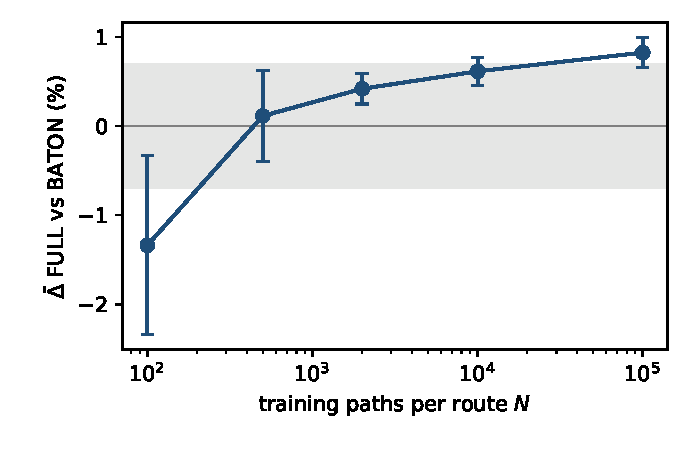
\includegraphics[width=0.6\textwidth]{figures/curve.pdf}}
{Data-size curve of experiment A: $\bar\Delta$ of \Full{} vs \Baton{} at equal
paths, with 95\% intervals; the shaded band is $\pm\delta$.\label{fig:curve}}
{}
\end{figure}

The advantage needs data (Figure~\ref{fig:curve}). With 100 paths per route
\Full{} is worse than \Baton{} ($\bar\Delta = $ \ASone{}, S1). The two are
equivalent at 500 paths (\AStwo{}) and the gain grows from there: \ASthree{}
at 2{,}000, \ASfour{} at $10^4$ and \APrim{} at $10^5$. Under the
pre-specified classes, the gains at 2{,}000 and $10^4$ paths are significant
but smaller than $\delta$, and only the gain at $10^5$ is a win. A plausible
reason for the small-sample loss is that the isotonic regressor's monotone
shape regularises \Baton{} for free while the networks are unconstrained; we
did not test this. An operator with a few hundred days of history per route
should keep the scalar policy; the rich state pays clearly only with
simulation-scale data, which a fitted demand model can supply.

\subsection{Against published methods}

\begin{table}[t]
\TABLE{Experiment B: \Full{} vs each published method on B's test stream
($n = 20$, 2 replicates, $\delta = $ \Margin{}).\label{tab:expb}}
{\scriptsize\begin{tabular}{llllllrll}
\toprule
arm & status & $\bar\Delta$ (\%) & CI95 & Holm CI & CI90 & \textsc{Full} better & $p$ & class \\
\midrule
\textsc{Alp-Z} & family & +11.33 & [+8.76, +13.91] & [+7.94, +14.72] & [+9.21, +13.46] & 20/20 & $7.6\times10^{-6}$ & win \\
\textsc{Rlsm} & family & +0.16 & [+0.09, +0.24] & [+0.06, +0.26] & [+0.10, +0.22] & 17/20 & 0.0003 & equivalent \\
\textsc{Dqn} & family & +0.16 & [+0.11, +0.21] & [+0.09, +0.22] & [+0.11, +0.20] & 19/20 & $1.1\times10^{-5}$ & equivalent \\
\textsc{Ppo} & family & +1.68 & [+0.46, +2.90] & [+0.07, +3.29] & [+0.67, +2.69] & 20/20 & $7.6\times10^{-6}$ & win \\
\textsc{Thr} & descriptive & +11.01 & [+8.48, +13.54] & -- & [+8.92, +13.10] & 20/20 & $1.9\times10^{-6}$ & -- \\
\bottomrule
\end{tabular}
}
{Family: Holm over four methods; classes use the 95\% interval and Holm $p$
(win) or the unadjusted 90\% interval (equivalent). \Thr{} failed its
development bug gate and is reported without adjustment or class.}
\end{table}

\begin{figure}[t]
\FIGURE{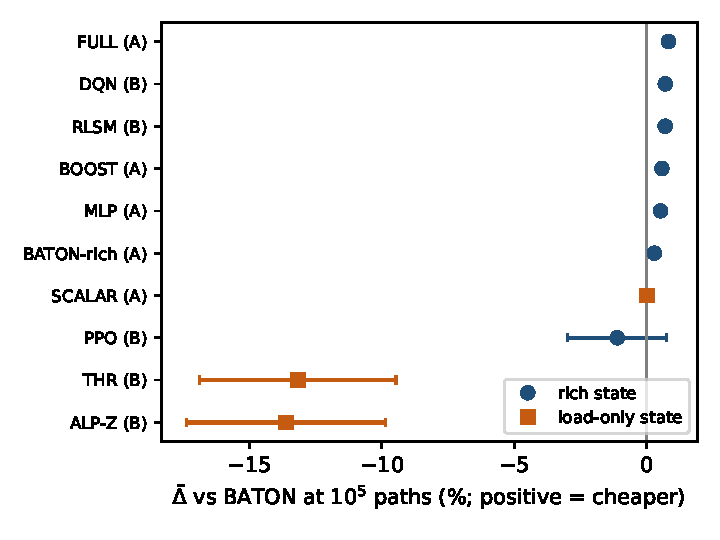
\includegraphics[width=0.62\textwidth]{figures/forest.pdf}}
{Every method against \Baton{} at $10^5$ paths ($\bar\Delta$, 95\% intervals;
positive = cheaper than \Baton{}). (A) and (B) mark the experiment and test
stream. Circles: rich state; squares: load-only state.\label{fig:forest}}
{Descriptive: these contrasts are outside the pre-specified families.}
\end{figure}

Table~\ref{tab:expb} gives the family of experiment B. The two methods that
see the rich state and learn a continuation value are equivalent to \Full{}:
\Rlsm{} (\BRlsm{}, 90\% interval \BRlsmCIn{}) and \Dqn{} (\BDqn{},
\BDqnCIn{}). Both are significantly but immaterially dearer, by
\ShareRlsm{} and \ShareDqn{} of \Full{}'s gain over \Baton{} on this stream,
and both are cheaper than \Baton{} (\BRlsmVsBaton{} and \BDqnVsBaton{}).
\Rlsm{} needs no gradient descent and fits in under a minute per route
(Table~\ref{tab:compute}). Our TD learner reaches the same cost as regression
on realised costs. We note that with a known handoff value and an
always-continue behaviour policy, its targets are close to those of
fitted value iteration, so this agreement is less surprising than it may seem.

The two methods that compute the continuation value from marginals lose
heavily: \Full{} is cheaper than \Alpz{} by \BAlpz{} \BAlpzCI{} of \Alpz{}'s
cost, on all 20 instances, and cheaper than \Thr{} by \BThr{}. Both are also
about 13\% dearer than \Baton{} (\BAlpzVsBaton{} and \BThrVsBaton{} of
\Baton{}'s cost), although \Baton{} observes exactly the same state, the net
load. The loss is therefore not caused by the load-only state, which costs
\Baton{} less than 1\% against \Full{}; it is caused by the estimator.
\Baton{} fits its continuation value to realised costs, which absorbs the
dependence between stops, while \Thr{} and \Alpz{} compute it from the
marginals under an independence assumption that is false on these instances.
The costs of \Thr{} and \Alpz{} differ by only \ThrAlpzGap{}, as expected of two
solutions of the same DP on different grids.

Our \Ppo{} adaptation is the one rich-state learner that falls short: against
it \Full{} has $\bar\Delta = $ \BPpo{} \BPpoCI{}, a win on all 20 instances,
and against \Baton{} \Ppo{} itself has $\bar\Delta = $ \BPpoVsBaton{}. Its
tuning record shows the same pattern: on the six tuning routes every
configuration was dearer than \Baton{}. A likely reason is that a policy
gradient must locate the decision boundary through sampled actions, while
regression and Q-learning use every realised cost directly; we did not test
larger budgets or variance-reduction devices, so the result concerns this
adaptation at this budget. Its median fit time, \PpoHours{} hours per route on
the CPU, is about nine times that of \Full{} and more than two hundred times
that of \Rlsm{} or \Dqn{}.

\subsection{Mechanism: the independence world}\label{sec:indep}

\begin{table}[t]
\TABLE{Independence world: each stop's training and test values permuted
by its own seeded permutation, which keeps every marginal and removes all
dependence between stops (12 routes, 10 instances, one replicate;
descriptive).\label{tab:indep}}
{\scriptsize\begin{tabular}{lllrl}
\toprule
comparison & $\bar\Delta$ (\%) & CI95 & \textsc{Full} better & $p$ \\
\midrule
\textsc{Full} vs none & +12.25 & [+7.82, +16.67] & 10/10 & 0.002 \\
\textsc{Full} vs \textsc{Baton} & +0.09 & [-0.39, +0.56] & 4/10 & 0.375 \\
\textsc{Full} vs oracle & -64.99 & [-84.65, -45.33] & 0/10 & 0.002 \\
\textsc{Full} vs \textsc{Thr} & -0.01 & [-0.31, +0.28] & 2/10 & 0.375 \\
\textsc{Full} vs \textsc{Alp-Z} & -0.03 & [-0.35, +0.28] & 4/10 & 0.625 \\
\bottomrule
\end{tabular}
}{}
\end{table}

If the rich state pays because the load is not a sufficient statistic, its
gain should vanish when stops are made independent, and the methods that
assume independence should recover. We tested this on twelve pre-selected
routes by permuting each stop's training and test values with its own seeded
permutation, which keeps every marginal and removes all dependence across
stops; every method was trained and evaluated in the permuted world. There
\Full{} is indistinguishable from \Baton{} (\BIndBaton{} \BIndBatonCI{}), from
\Thr{} (\BIndThr{} \BIndThrCI{}) and from \Alpz{} (\BIndAlpz{}
\BIndAlpzCI{}); all three intervals lie inside $\pm\delta$, and \Full{} still
beats never handing off by \BIndNone{} (Table~\ref{tab:indep}). The rich state
has nothing to add when the load is sufficient, and the independence-based
methods are as good as the learners when their assumption holds. This test is
descriptive (one replicate, ten instances) and covers only the two endpoints,
full dependence and none; it supports, but does not by itself prove, the
attribution of Section~\ref{sec:results}. \Thr{}'s own-model check, which
compares its simulated and predicted costs in this world, failed on 7 of 62
development routes (Section~\ref{sec:limits}), so the agreement with \Thr{}
should be read with that caveat.

\subsection{Variability and compute}

\begin{table}[t]
\TABLE{Fit time per route and replicate at $10^5$ paths (seconds,
median and maximum over route-replicates).\label{tab:compute}}
{\begin{tabular}{llrr}
\toprule
method & experiment & median (s) & max (s) \\
\midrule
\textsc{Full} & A & 2{,}356 & 5{,}929 \\
\textsc{Mlp} & A & 122 & 216 \\
\textsc{Boost} & A & 43 & 70 \\
\textsc{Thr} & B & 320 & 518 \\
\textsc{Alp-Z} & B & 0.5 & 0.9 \\
\textsc{Rlsm} & B & 42 & 77 \\
\textsc{Dqn} & B & 88 & 181 \\
\textsc{Ppo} & B & 21{,}351 & 45{,}161 \\
\bottomrule
\end{tabular}
}
{\Dqn{} trains on the GPU; all other methods and every evaluation run on the
CPU. \Full{} is shown from A; its median in B is \FullMinutesB{} minutes.
\Alpz{} solves an LP on a 401-point lattice; \Thr{} runs its recursion with all
$10^5$ marginal samples on a 2{,}001-point grid. \Baton{} fits in about a
second.}
\end{table}

Training noise is small: the mean over routes of the between-replicate
standard deviation of a route's cost is \RepSdFull{} for \Full{},
\RepSdBaton{} for \Baton{}, \RepSdRlsm{} for \Rlsm{}, \RepSdDqn{} for \Dqn{}
and \RepSdPpo{} for \Ppo{}. The cheapest rich-state learners (\Boost{} and
\Rlsm{} at well under a minute, \Dqn{} at about a minute and a half on a GPU)
fit far faster than \Full{} (Table~\ref{tab:compute}).

%% ==========================================================================
\section{Discussion}\label{sec:discussion}

\paragraph{State and estimator, not architecture.} Two lessons come out of
the comparison. First, what the policy observes decides most of the gain: every
learner we tried on the rich state reaches nearly the same cost, and no learner
on the load beats the load-only DP. Second, how the continuation value is
estimated decides the losses: fitting it to realised costs is robust to the
dependence structure, while computing it from marginals is exact only when
stops are independent and costs about 13\% when they are not. The
architecture is a distant third. For an operator this means recording what
the driver already observes, how much was delivered and how much was picked
up at each stop, and fitting the simplest regressor that uses it; boosted
trees and randomized networks fit in under a minute per route.

\paragraph{When the rich state pays.} Two conditions are needed: dependence
across stops that the load hides (in the independence world the gain is zero),
and enough data. The rich state stops losing at about \Crossover{} paths per
route and becomes a clear gain only with simulation-scale data. In practice
those paths would come from a demand model fitted to history, which moves the
problem to fitting the dependence structure well.

\paragraph{Value-based learners and policy gradients.} Regression on realised
costs and double Q-learning reach the same cost; our \Ppo{} adaptation does
not, at a budget slightly above its source's. A two-action stopping problem
with known handoff prices favours value-based methods: the value of stopping is
known exactly, so only one function has to be learned, while a policy-gradient
method must find the boundary through sampled actions.

\paragraph{The reference policy.} \Baton{} remains a strong default. At large
samples it matches the best policy in its information class (S7), it is better
with little data, and it fits in about a second. The rich state is an upgrade
worth about \APrim{} of recourse cost when the data and the dependence are
there.

%% ==========================================================================
\section{Limitations}\label{sec:limits}

We list what the design does not support. (i) We measure recourse cost only;
we do not measure total route cost, of which recourse is one part, so the
operational value of the gain depends on the share of recourse in a given
operation. (ii) All results use one demand generator family on two instance
classes of one benchmark. We did not vary the copula correlation, the
coefficient of variation or the price ratio, and the independence world
shows that the gain can vanish; how it scales with dependence is open. (iii)
We did not run a model-based DP on an augmented state such as $(W_k, P_k,
D_k)$ under a fitted dependence model, which would separate state and
estimator further. (iv) \Dqn{} was trained for one pass over $8 \times 10^4$
paths per route, far fewer realisations than the millions used in its line of
work \citep{dastpak2026deep}; it matches \Full{} here, and a larger budget
could only help it, but we did not test whether it would then beat \Full{}.
\Ppo{} was trained at about its source's episode count and not beyond. Both
deep methods replace their sources' graph encoders by a set encoder. (v) Deep
optimal stopping was removed by a pre-specified compute cut after it had been
tuned on development data, and experiment B used two training replicates
instead of three. (vi) \Thr{} failed its own-model check on development data:
on 7 of 62 routes its simulated cost left a band of four standard errors around
its predicted value. On five of these routes the simulated cost was exactly
zero on all development days, so the band had zero width; the other two
deviations were genuine (about five standard errors), and the simulated cost
was below the predicted value on most routes. \Thr{} is therefore reported
descriptively. (vii) The \Dqn{} tuning scores of one configuration varied by up
to 0.28 points between passes, so the chosen configuration is not sharply
identified. (viii) The pre-specification is a time-stamped, hashed record in
the code repository, not an external registry.

%% ==========================================================================
\section{Conclusion}\label{sec:conclusion}

For in-route handoff with stochastic pickups and deliveries, what a policy
observes matters far more than how it learns. Regression on the rich state, by
a transformer, a perceptron, boosted trees or randomized features, and double
Q-learning all reach nearly the same cost, \APrim{} below the
Longstaff--Schwartz policy on the load. Methods that compute the continuation
value from marginals under independence lose about 13\% on correlated demand,
and an independence-permuted world removes that loss. Future work should vary
the dependence structure, add model-based policies on augmented states, and
test whether the same lesson holds when standby vehicles are shared across
routes or the route itself can change.

\ACKNOWLEDGMENT{Blinded for peer review.}

\bibliographystyle{informs2014trsc}
\bibliography{references}

%% ==========================================================================
\begin{APPENDICES}

\section{State Features}\label{app:features}

The global vector at stop $k$ has twelve entries: $W_k/B$; $\max_{j \le k}
W_j/B$; $k/m$, $(m-k)/m$ and $m/22$; $H_k/E_0$ and $E_k/E_0$; $P_k/B$ and
$D_k/B$; the mean standardised pickup and delivery deviations over the stops
served; and $(p_k - d_k)/B$. Each remaining stop $j > k$ has a token of eleven
entries: the historical means and standard deviations of its pickup and
delivery divided by $B$; $(j-k)/m$ and $j/m$; its handoff and emergency prices
divided by $E_0$; an indicator of the last stop; the expected net load after
it, $(W_k + \sum_{i=k+1}^{j}\hat\mu^g_i)/B$; and the standardised distance of
that load to the slack. \Scalar{} sets the six history entries (running
maximum, $P_k$, $D_k$, the two deviations and the last increment) to zero.
All statistics are computed from the fitting paths and clipped to $[-5, 5]$.
\Mlp{} and \Rlsm{} use the twelve global entries and three token summaries: the
smallest standardised distance to the slack, its position, and the smallest
remaining handoff price.

\section{Adaptations of the Published Methods}\label{app:adapt}

\paragraph{\Thr{}.} Empirical marginals of the training paths instead of a
parametric demand distribution; the common tie rule (hand off when the
continuation value is within $10^{-6}E_0$ of the handoff price), which changes
decisions only at the threshold.

\paragraph{\Alpz{}.} (1) Load lattice instead of integer capacities; (2)
handoff and breach are terminal at fixed prices, whereas the source's
restocking and outsourcing continue the route; (3) HiGHS instead of Gurobi;
(4) no routing part (no travelling-salesman bound, next-customer choice or
heuristic pool). The source tunes only the heuristic pool and the outsourcing
price, neither of which exists here.

\paragraph{\Rlsm{}.} Hidden layer redrawn at every stop (the source's
``reinit'' variant), leaky-ReLU slope 0.5 as in the released code, and a ridge
penalty added to the least-squares solve and tuned.

\paragraph{\Dqn{}.} Rich state with a masked set encoder instead of the 2023
paper's fixed-size observation. Only the continuation value is learned; the
handoff value is the known price. Discount $\gamma = 1$ and targets scaled by
$E_0$. The behaviour policy always continues (off-policy, no
$\varepsilon$-greedy). Minibatch 256 with one update per 32 stored
transitions (the paper uses minibatch 32, the released code 128), buffer
50{,}000 as in the paper, Huber loss and gradient-norm clipping at 10.

\paragraph{\Ppo{}.} Graph convolution layers dropped (fixed route); actions
\{continue, handoff\} instead of the next node; rewards are the negative
prices, without the source's coverage shaping, which would change the optimal
stopping rule; initial handoff probability 0.05; value coefficient 0.5 and no
advantage normalisation. The paper describes a value network and a GRU; the
released code has no value network, and we follow the paper.

\section{Protocol Deviations}\label{app:dev}

Deviations were logged with date and reason in the repository before the
affected test stream was read. In B, the compute trigger applied three
pre-specified cuts (no \Dos{}, six tuning routes, two replicates). The
development gate report was produced by running the frozen gate functions per
method in parallel processes after a first sequential run stopped on an
operator error in its final step; the code was unchanged. One analysis-only
patch in A (the grid of the data-size curve) was registered by hash before A's
test stream was opened by a learned policy. The \Baton{}-only pass on A's test
stream is described in Section~\ref{sec:protocol}.

\end{APPENDICES}

\end{document}
